
% utf-8 ru, unix eolns
\documentclass[12pt,a4paper,oneside]{extarticle}
    \righthyphenmin=2 %минимально переносится 2 символа %%%
    \sloppy

% Рукопись оформлена в соответствии с правилами оформления 
% электронной версии авторского оригинала, 
% принятыми в Издательстве МГТУ им. Н.Э. Баумана.

\usepackage{geometry} % А4, примерно 28-31 строк(а) на странице 
    \geometry{paper=a4paper}
    \geometry{includehead=false} % Нет верх. колонтитула
    \geometry{includefoot=true}  % Есть номер страницы
    \geometry{bindingoffset=0mm} % Переплет    : 0  мм
    \geometry{top=20mm}          % Поле верхнее: 20 мм
    \geometry{bottom=25mm}       % Поле нижнее : 25 мм 
    \geometry{left=25mm}         % Поле левое  : 25 мм
    \geometry{right=25mm}        % Поле правое : 25 мм
    \geometry{headsep=10mm}  % От края до верх. колонтитула: 10 мм
    \geometry{footskip=20mm} % От края до нижн. колонтитула: 20 мм 

\usepackage{cmap}
\usepackage[T2A]{fontenc} 
\usepackage[utf8x]{inputenc}
\usepackage[english,russian]{babel}
\usepackage{misccorr}

\usepackage{amsmath}
\usepackage{amsfonts}
\usepackage{amssymb}

%\usepackage{cm-super} %человеческий рендер русских шрифтов

\setlength{\parindent}{1.25cm}  % Абзацный отступ: 1,25 см
\usepackage{indentfirst}        % 1-й абзац имеет отступ

\usepackage{setspace}   

\onehalfspacing % Полуторный интервал между строками

\makeatletter
\renewcommand{\@oddfoot }{\hfil\thepage\hfil} % Номер стр.
\renewcommand{\@evenfoot}{\hfil\thepage\hfil} % Номер стр.
\renewcommand{\@oddhead }{} % Нет верх. колонтитула
\renewcommand{\@evenhead}{} % Нет верх. колонтитула
\makeatother

\usepackage{fancyvrb}


\usepackage[pdftex]{graphicx}  % поддержка картинок для пдф
\graphicspath{ {./pictures/} }
\usepackage{rotating}
%\DeclareGraphicsExtensions{.jpg,.png}




\renewcommand{\labelenumi}{\theenumi.} %меняет вид нумерованного списка

\usepackage{perpage} %нумерация сносок 
\MakePerPage{footnote}

\usepackage[all]{xy} %поддержка графов

\usepackage{listings} %листинги
\renewcommand{\lstlistingname}{Листинг}
\lstset{
  basicstyle=\small,
  breaklines=true
  }


\usepackage{url}


\usepackage{tikz} %для рисования графиков
\usepackage{pgfplots}

\usepackage{gensymb}

\usepackage{ccaption}%изменяет подпись к рисунку
\makeatletter 
\renewcommand{\fnum@figure}[1]{Рисунок~\thefigure~---~\sffamily}
\makeatother

\begin{document}
\pgfplotsset{compat=1.8}

\thispagestyle{empty}
\newpage
{
\centering


\textbf{
МОСКОВСКИЙ ГОСУДАРСТВЕННЫЙ ТЕХНИЧЕСКИЙ УНИВЕРСИТЕТ ИМЕНИ Н. Э. БАУМАНА \\
Факультет информатики и систем управления \\
Кафедра теоретической информатики и компьютерных технологий}
\bigskip
\bigskip
\bigskip
\bigskip
\bigskip
\bigskip
\bigskip

\vfill


Лабораторная работа №4 \\
по курсу <<Математическое моделирование>>

\bigskip

{\large <<Определение выброса методом исключения одной точки>>}
\bigskip

\vfill



\hfill\parbox{4cm} {
Выполнил:\\
студент ИУ9-111 \hfill \\
Выборнов А. И.\hfill \medskip\\
Руководитель:\\
Домрачева А. Б.\hfill
}


\vspace{\fill}

Москва \number\year
\clearpage
}



\clearpage


\section{Постановка задачи}
    Рассматриваются 6 станций чешского метрополитена. Для каждой станции, вручную была посчитана следующая информация с точностью до месяца:
    \begin{itemize}
        \item Среднее число пассажиров, вошедших с данной станции в метрополитена в день.
        \item Среднее число пассажиров, вышедших с данной станции в день.
    \end{itemize}

    Данные для 6 станций (A0, A1, B0, B1, C0, C1) приведены в таблице~\ref{tabular:data}. Строки соответствуют месяцам, столбцы станциям метро, причём префикс "th" \space соответствует вошедшим пассажирам, а префикс "r" \space вышедшим.
    \begin{table}[ht!]
        \caption{Данные о числе пассажиров проходящих через станции Пражского метро}
        \centering
        \label{tabular:data}
        \small
        \begin{tabular}{|c|c|c|c|c|c|c|c|c|c|c|c|c|}
        \hline
        m/s & thA0 & rA0 & thA1 & rA1 & thB0 & rB0 & thB1 & rB1 & thC0 & rC0 & thC1 & rC1 \\ \hline
        1 & 16551 & 14899 & 30746 & 27320 & 32822 & 29553 & 21002 & 18793 & 17084 & 15365 & 4544 & 3118 \\ \hline
        2 & 16810 & 14292 & 22558 & 20155 & 25314 & 22567 & 40022 & 35436 & 29096 & 25876 & 17519 & 16162 \\ \hline
        3 & 14434 & 13046 & 28001 & 24916 & 36918 & 32720 & 35118 & 31145 & 38639 & 34226 & 38841 & 34819 \\ \hline
        4 & 20891 & 18696 & 32958 & 29255 & 46677 & 41259 & 20283 & 18164 & 23690 & 21145 & 37324 & 33492 \\ \hline
        5 & 13773 & 12468 & 28277 & 25159 & 16909 & 15212 & 41746 & 36944 & 29087 & 25868 & 16717 & 15461 \\ \hline
        6 & 14739 & 13313 & 36763 & 32398 & 21889 & 19569 & 40458 & 35817 & 21993 & 20494 & 40099 & 35920 \\ \hline
        7 & 24713 & 22040 & 34650 & 30735 & 34998 & 31040 & 19478 & 17460 & 30082 & 26738 & 42244 & 37797 \\ \hline
        8 & 10127 & 9278 & 33590 & 29808 & 23285 & 20791 & 22974 & 21353 & 18776 & 17263 & 22099 & 20170 \\ \hline
        9 & 14689 & 13269 & 12239 & 11126 & 21561 & 19282 & 25348 & 23430 & 34808 & 31290 & 40895 & 36617 \\ \hline
        10 & 13047 & 11833 & 35848 & 31784 & 37778 & 33472 & 25336 & 22586 & 26192 & 23751 & 17519 & 16162 \\ \hline
        11 & 16487 & 14843 & 38451 & 34061 & 29376 & 26120 & 23743 & 22025 & 18230 & 16784 & 38841 & 34819 \\ \hline
        12 & 14345 & 12968 & 18573 & 16668 & 32822 & 29553 & 29751 & 27282 & 37085 & 33283 & 37324 & 33492 \\ \hline
        \end{tabular}
    \end{table}

    Для обобщённых данных необходимо сравнить функции распределения для вошедших и вышедших, основываясь на критерии Колмогорова-Смирнова. Определить выброс, методом исключения одной точки.

\section{Решение}
    Область значений входных данных была отображена на интервал от 0 до 1. Область определения входных была разбита на 20 интервалов и, на основе этого, были посчитаны функции распределения.
    Для построенных функций распределения использовалась модификация критерия Колмогорова-Смирнова --- вместо функции $\max_i|x_i-y_i|$ используется функция $\sum_{i}|x_i-y_i|$. Это делается с целью получить интегральную характеристику расхождения функций распределения, что позволяет в рамках задачи получить более чувствительный критерий.

    Полученные функции распределения изображены на рисунке~\ref{pic:case1}.
    \begin{figure}[ht!]
    \center
        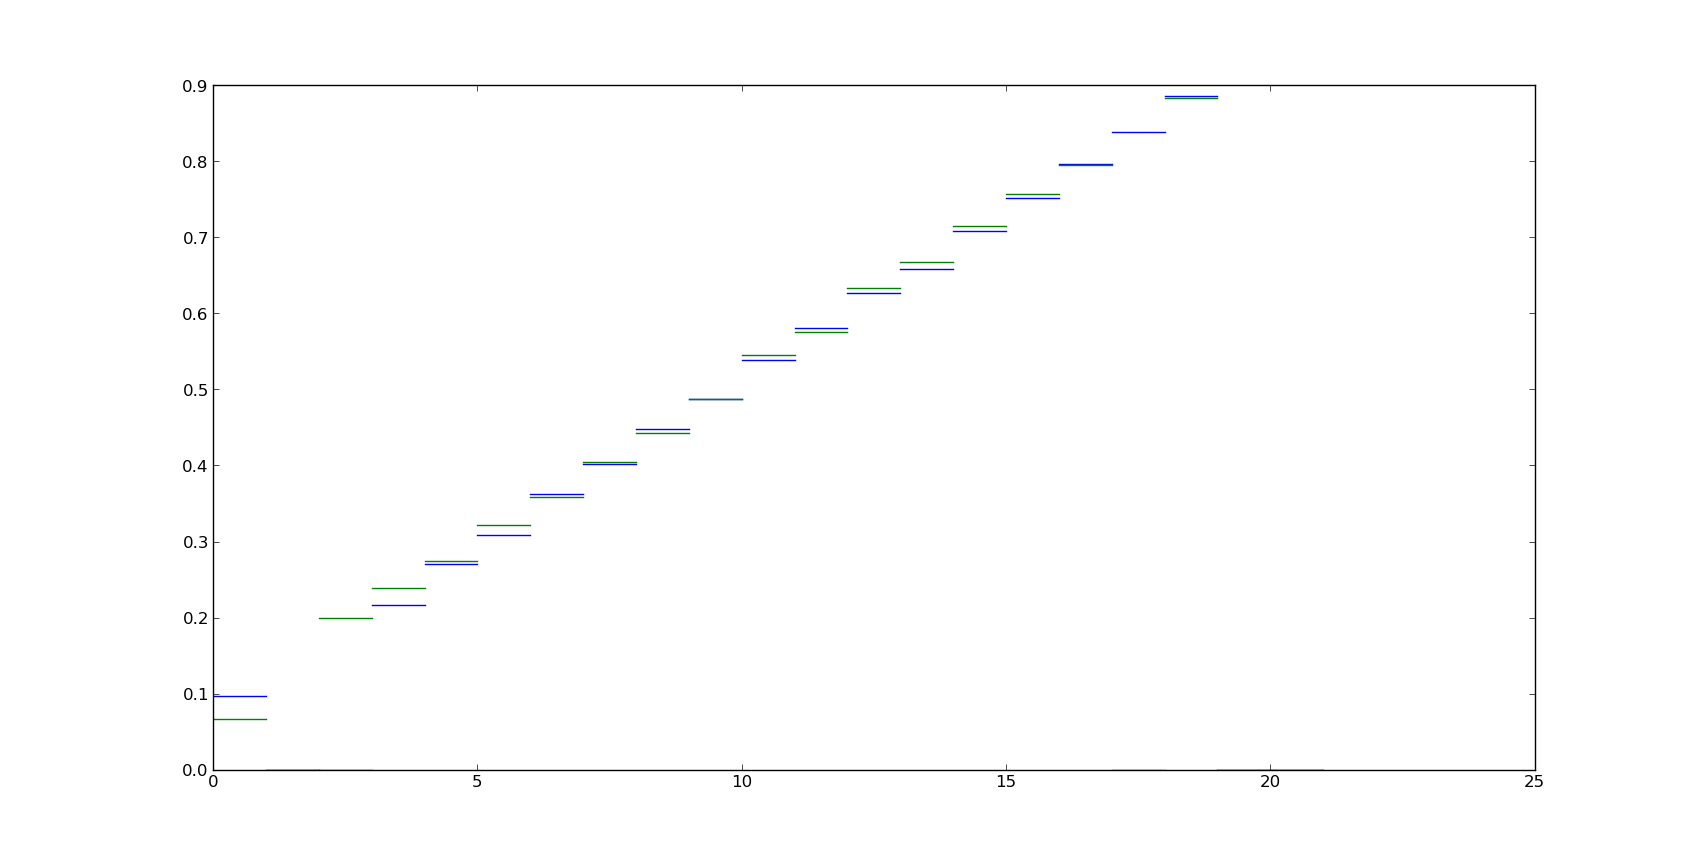
\includegraphics[scale=0.45]{figure_1.png}
        \caption{Функции распределения: синий график вошедшие пассажиры, зелёный график вышедшие}
        \label{pic:case1}
    \end{figure}
    Cогласно модифицированному критерию полученные функции распределения расходятся на значение: 1.16281626925.

    Попытаемся найти выброс методом исключения одной точки. Для этого посчитаем меру расхождения функций согласно модифицированному критерию Колмогорова-Смирнова для входных данных, последовательно исключая из них по одной точке. Результаты, отсортированные по мере расхождения, приведены в таблице~\ref{tabular:data1}.

    \begin{table}[ht!]
        \caption{Поиск выброса методом исключения одной точки}
        \centering
        \label{tabular:data1}
        \tiny
        \begin{tabular}{|c|c|c|}
        \hline
        кол-во вошедших для исключённой точки & кол-во вышедших для исключённой точки & мера расхождения \\ \hline
        17519 & 16162 & 1.0832150432 \\ \hline 
        42244 & 37797 & 1.15575747513 \\ \hline 
        37778 & 33472 & 1.15629878384 \\ \hline 
        38841 & 34819 & 1.15855455986 \\ \hline 
        38841 & 34819 & 1.15855455986 \\ \hline 
        32822 & 29553 & 1.15863648049 \\ \hline 
        35118 & 31145 & 1.15867968521 \\ \hline 
        38639 & 34226 & 1.15902746535 \\ \hline 
        21993 & 20494 & 1.15904603266 \\ \hline 
        10127 & 9278 & 1.16050892302 \\ \hline 
        36763 & 32398 & 1.16063853718 \\ \hline 
        26192 & 23750 & 1.1608474195 \\ \hline 
        29096 & 25876 & 1.16089210348 \\ \hline 
        37085 & 33283 & 1.16092704473 \\ \hline 
        40458 & 35817 & 1.16093632838 \\ \hline 
        14738 & 13313 & 1.16097132064 \\ \hline 
        32822 & 29553 & 1.1610998636 \\ \hline 
        21002 & 18793 & 1.16112557219 \\ \hline 
        25314 & 22567 & 1.16112557219 \\ \hline 
        28001 & 24916 & 1.16122277006 \\ \hline 
        40099 & 35920 & 1.16160398667 \\ \hline 
        29376 & 26119 & 1.16165754624 \\ \hline 
        30746 & 27320 & 1.16189254522 \\ \hline 
        16717 & 15461 & 1.16197625118 \\ \hline 
        20891 & 18696 & 1.16203501368 \\ \hline 
        21889 & 19569 & 1.1620832683 \\ \hline 
        13047 & 11833 & 1.16244527997 \\ \hline 
        23690 & 21145 & 1.16245135006 \\ \hline 
        24713 & 22040 & 1.16252454814 \\ \hline 
        40895 & 36617 & 1.16269183252 \\ \hline 
        21561 & 19282 & 1.162862407 \\ \hline 
        40022 & 35436 & 1.16290981997 \\ \hline 
        33590 & 29808 & 1.16297373439 \\ \hline 
        36918 & 32720 & 1.16307728289 \\ \hline 
        23285 & 20791 & 1.16320404053 \\ \hline 
        34998 & 31040 & 1.16326777642 \\ \hline 
        20283 & 18164 & 1.16328437989 \\ \hline 
        23743 & 22025 & 1.1633158015 \\ \hline 
        4544 & 3118 & 1.16363996442 \\ \hline 
        18573 & 16668 & 1.1637618762 \\ \hline 
        38451 & 34061 & 1.16377177196 \\ \hline 
        13773 & 12468 & 1.16422202941 \\ \hline 
        28276 & 25158 & 1.16422488592 \\ \hline 
        30082 & 26737 & 1.16440451451 \\ \hline 
        16810 & 14292 & 1.16452007566 \\ \hline 
        12239 & 11126 & 1.16478904671 \\ \hline 
        14345 & 12967 & 1.16495589752 \\ \hline 
        25347 & 23430 & 1.16508273168 \\ \hline 
        34808 & 31290 & 1.16509897808 \\ \hline 
        18776 & 17263 & 1.16535356457 \\ \hline 
        29086 & 25868 & 1.16561873544 \\ \hline 
        46677 & 41259 & 1.1660786081 \\ \hline 
        14434 & 13046 & 1.1663282467 \\ \hline 
        19478 & 17460 & 1.16664863495 \\ \hline 
        29751 & 27282 & 1.16684285214 \\ \hline 
        25336 & 22586 & 1.16701783891 \\ \hline 
        37324 & 33492 & 1.16704461869 \\ \hline 
        37324 & 33492 & 1.16704461869 \\ \hline 
        34650 & 30735 & 1.16772824283 \\ \hline 
        17084 & 15365 & 1.16782016125 \\ \hline 
        17519 & 16162 & 1.16794549064 \\ \hline 
        22974 & 21353 & 1.17095625254 \\ \hline 
        41746 & 36944 & 1.1714132942 \\ \hline 
        22099 & 20170 & 1.17327288243 \\ \hline 
        16487 & 14843 & 1.17568413423 \\ \hline 
        32958 & 29255 & 1.1761222515 \\ \hline 
        14689 & 13269 & 1.18100509887 \\ \hline 
        18230 & 16784 & 1.18655529847 \\ \hline 
        35848 & 31784 & 1.35960840814 \\ \hline 
        22558 & 20155 & 1.82476255258 \\ \hline 
        16909 & 15211 & 2.46879736834 \\ \hline 

        \end{tabular}
    \end{table}

    Из полученных метрик минимальное значение 1.0832150432 достигается в точке (4544.0, 3118.0).
    Исключая из входных данных точку (4544.0, 3118.0), мы получили функции распределения, изображённые на рисунке~\ref{pic:case2}.
    \begin{figure}[ht!]
        \center
        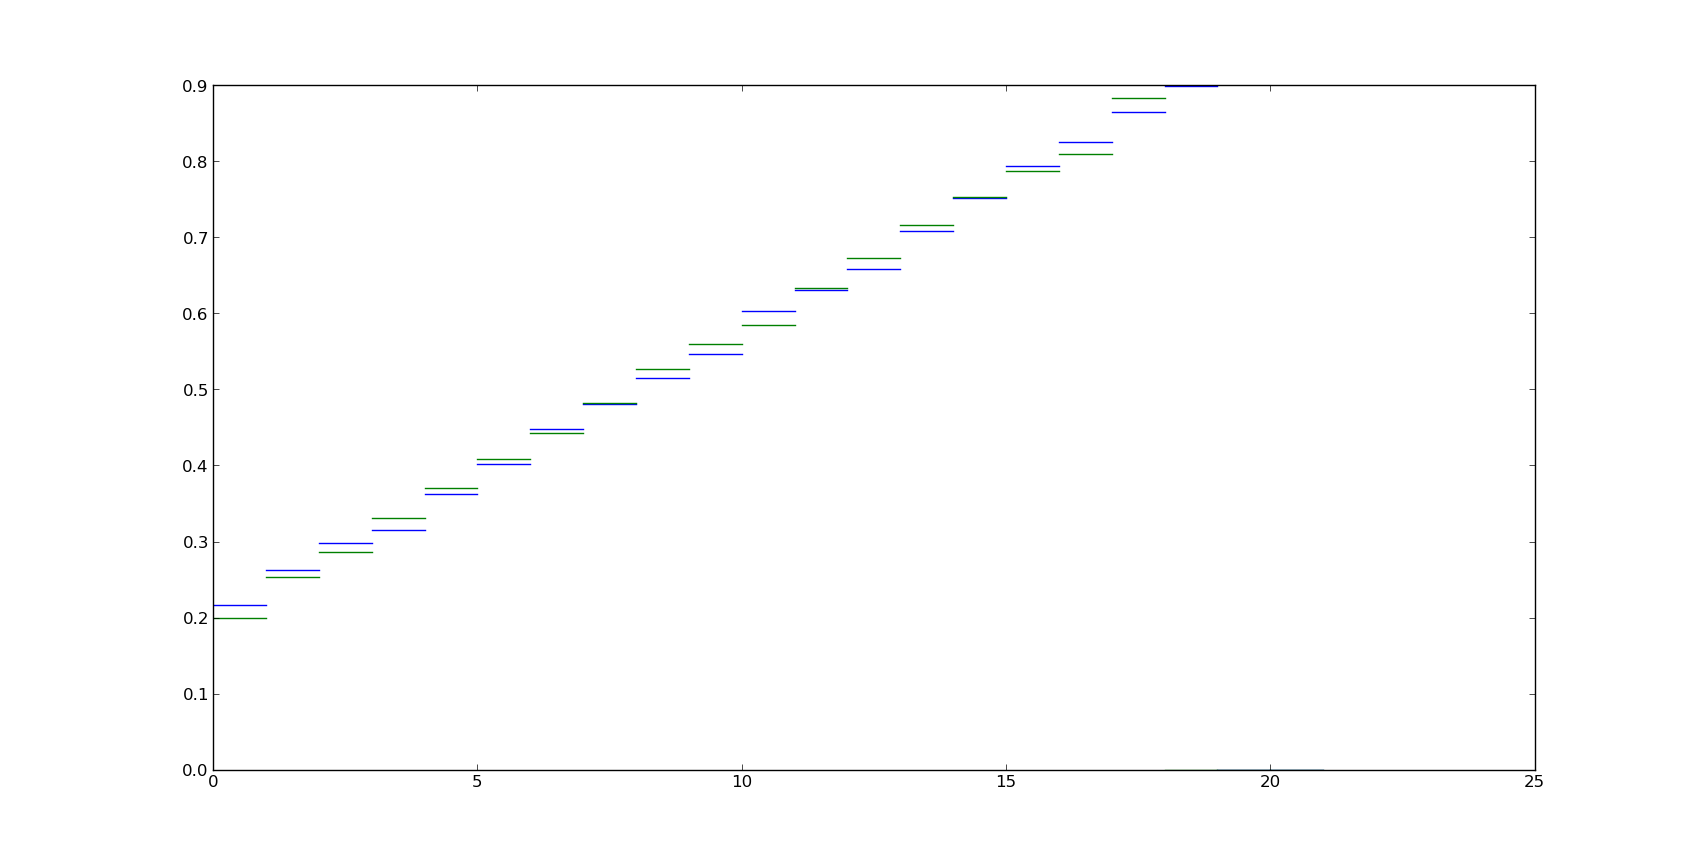
\includegraphics[scale=0.45]{figure_2.png}
        \caption{Функции распределения: синий график вошедшие пассажиры, зелёный график вышедшие}
        \label{pic:case2}
    \end{figure}

    Исключением точки (4544.0, 3118.0) мы не только снизили значение коэффициента расхождения функций распределений, но и, как видно из полученного рисунка, визуально наблюдается соответствие функций распределения исходных выборок. Также если рассмотреть минимальные коэффициенты расхождения из таблицы видно, что второе по минимальности значение меры расхождения уже на порядок ближе к значению функции расхождения для исходных данных. Поэтому полагаем, что это точка, является точкой выброса.
\end{document}
